%%This is a very basic article template.
%%There is just one section and two subsections.

\documentclass[20pt]{beamer}

\usepackage[ngerman,english]{babel}
\usepackage{tikz}
\usepackage[normalem]{ulem}
\geometry{paperwidth=10in, paperheight=7.5in}

\usepackage[utf8]{inputenc}

\usepackage[mpidr]{./mpidr/beamerthemeMPIDR}
\usepackage{animate}
%% Declaring title and author
\title{Birth, Death, \& Thermodynamics}
\subtitle{Tim Riffe}		%%

%%	the institute's logo
\renewcommand{\mylogo}{\includegraphics[width=4.7in]{mpidr_logo_colour_en}}
\usepackage{color}
\definecolor{mygray}{rgb}{0.8,0.8,0.8}

\defbeamertemplate{description item}{align left}{\insertdescriptionitem\hfill}
%%	should be the very last package to be loaded
\usepackage{hyperref}

%%%%%%%%%%%%%%%%%%%%%%%%%%%%%%%%%%
%%	Beginning of the document		%%
%%%%%%%%%%%%%%%%%%%%%%%%%%%%%%%%%%
\begin{document}

%%	titlepage - fixed frame:
%%	========================

\begin{frame}
	\titlepage
\end{frame}

\begin{frame}
\frametitle{About that title}
\onslide<1>\begin{block}{On the one hand}
Birth and death are events experienced by individuals. Both are conditioned by
randomness, circumstance, and agency.
\end{block}
\vspace{1em}
\onslide<2>\begin{block}{On the other hand}
Birth and death have very strong and steady age patterns. It's easy to think
there might be \textit{laws}.
\end{block}
\end{frame}

\begin{frame}
\frametitle{Laws? two kinds:}
\onslide<1>\begin{block}{On the one hand}
You can \textit{only} enter a population via birth or in-migration. You can \textit{only}
leave a population via death or out-migration. (conservation)
\end{block}
\onslide<2>\begin{block}{On the other hand}
The forces of demographic change (mostly fertility and mortality) are bounded
and very empirically regular, ergo law-abiding.
\end{block}
\end{frame}

\begin{frame}
\frametitle{laws for mortality}
\vspace{-1em}
\begin{center}
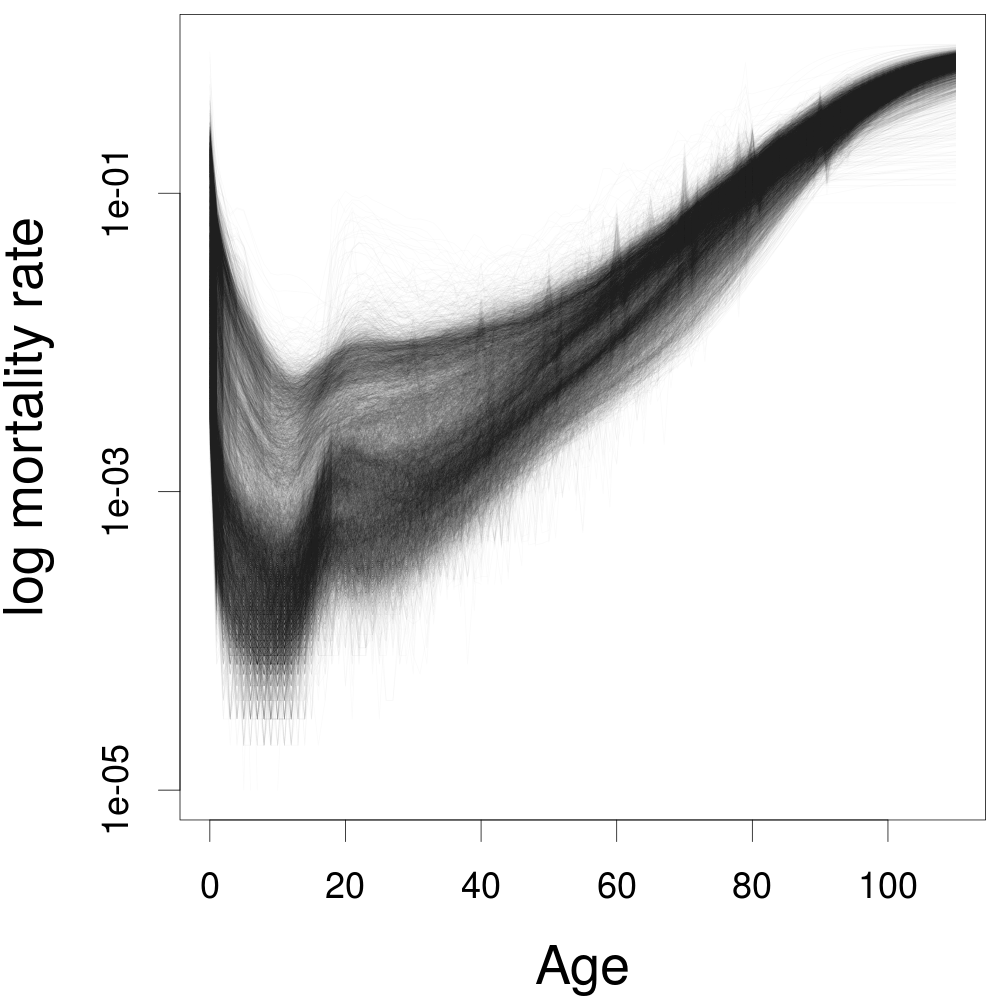
\includegraphics[height=6in]{Figures/Mortality1.png}
\end{center}
\end{frame}

\begin{frame}
\frametitle{laws for mortality}
\vspace{-1em}
\begin{center}
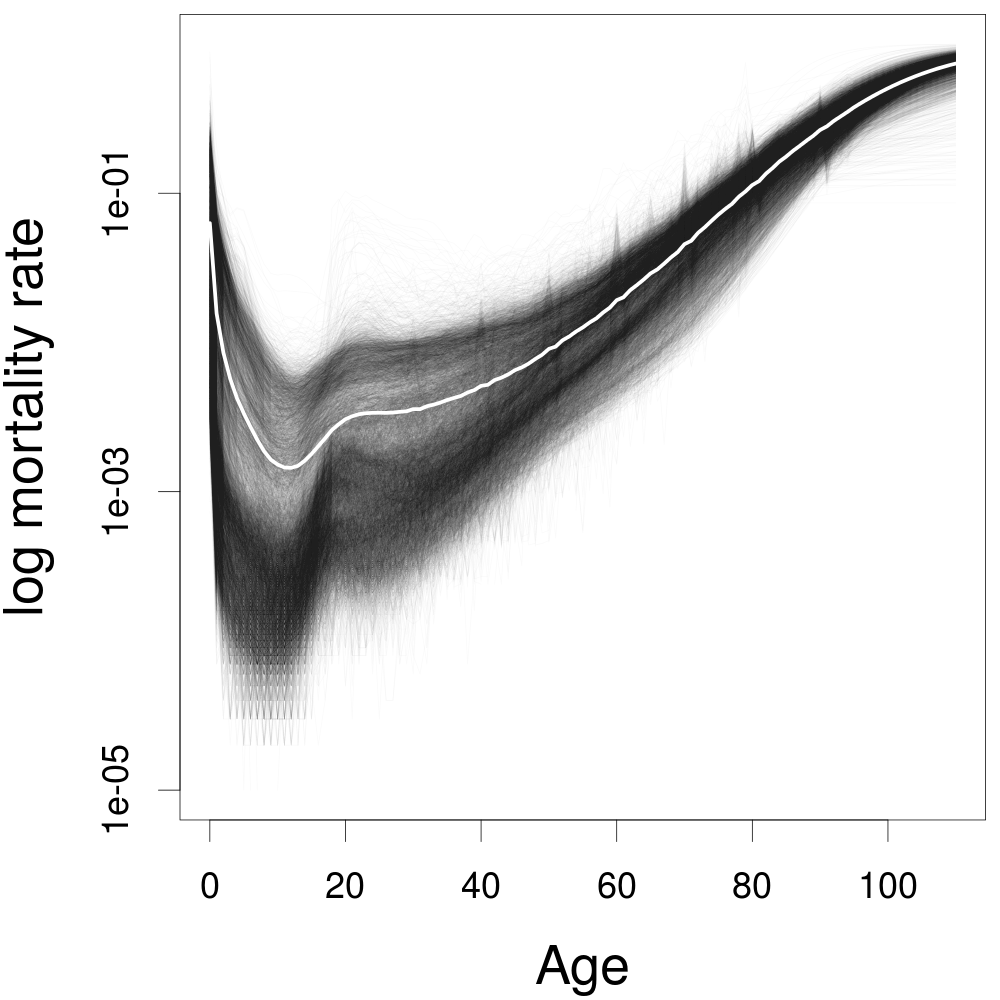
\includegraphics[height=6in]{Figures/Mortality2.png}
\end{center}
\end{frame}

\begin{frame}
\frametitle{laws for mortality}
\vspace{-1em}
\begin{center}
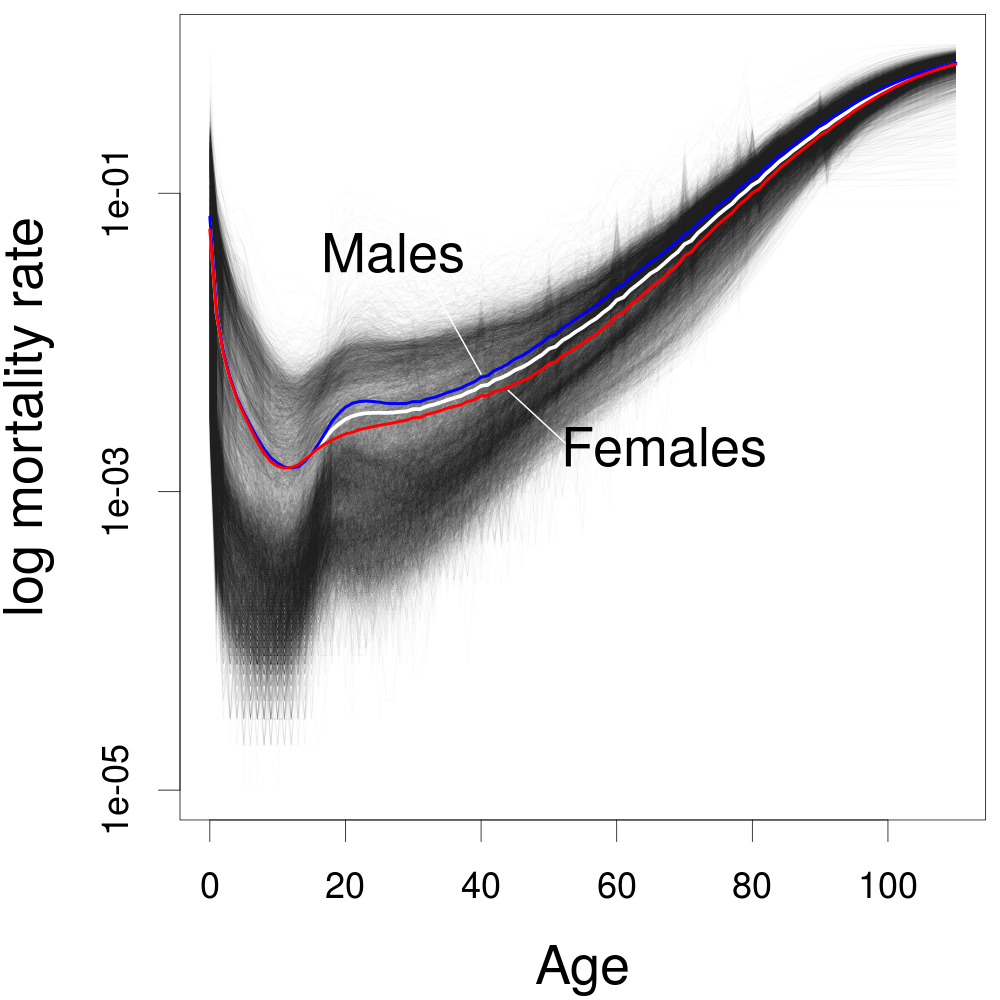
\includegraphics[height=6in]{Figures/Mortality3.png}
\end{center}
\end{frame}

\begin{frame}
\frametitle{laws for fertility}
\vspace{-1em}
\begin{center}
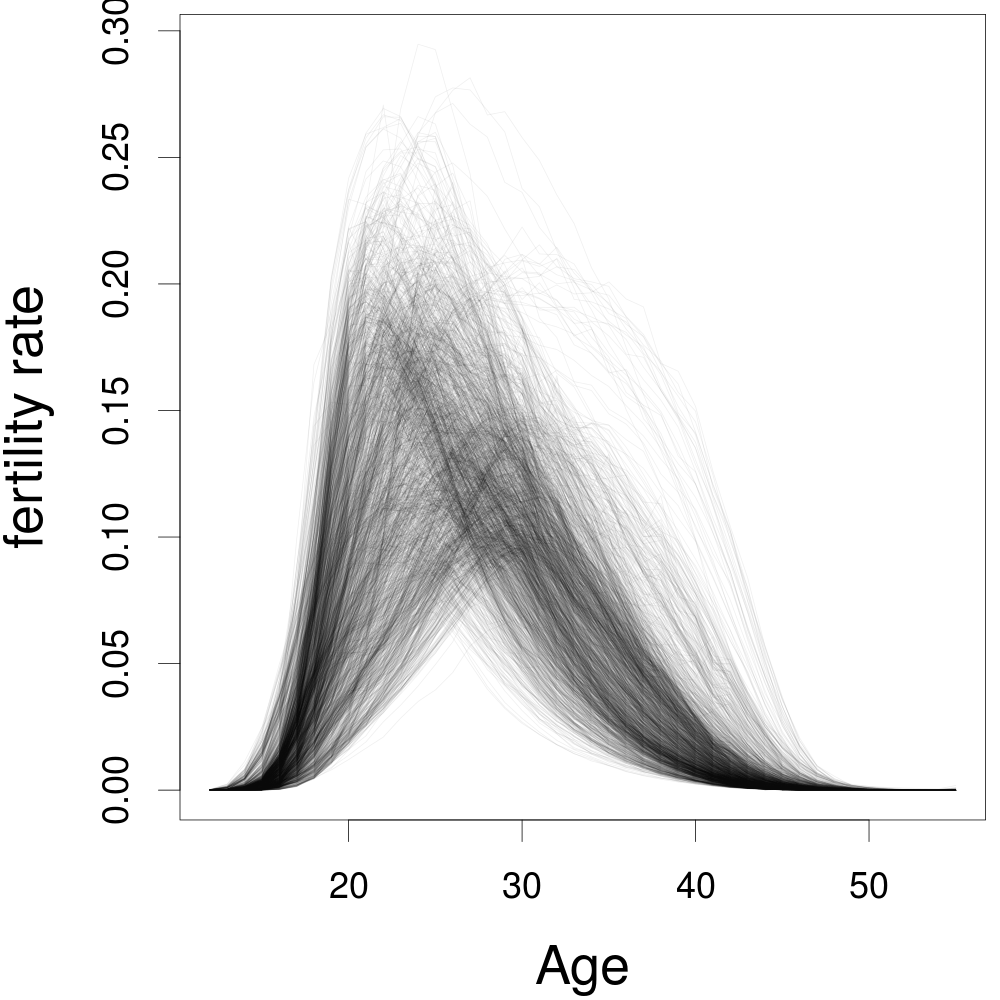
\includegraphics[height=6in]{Figures/Fertility1.png}
\end{center}
\end{frame}

\begin{frame}
\frametitle{laws for fertility}
\vspace{-1em}
\begin{center}
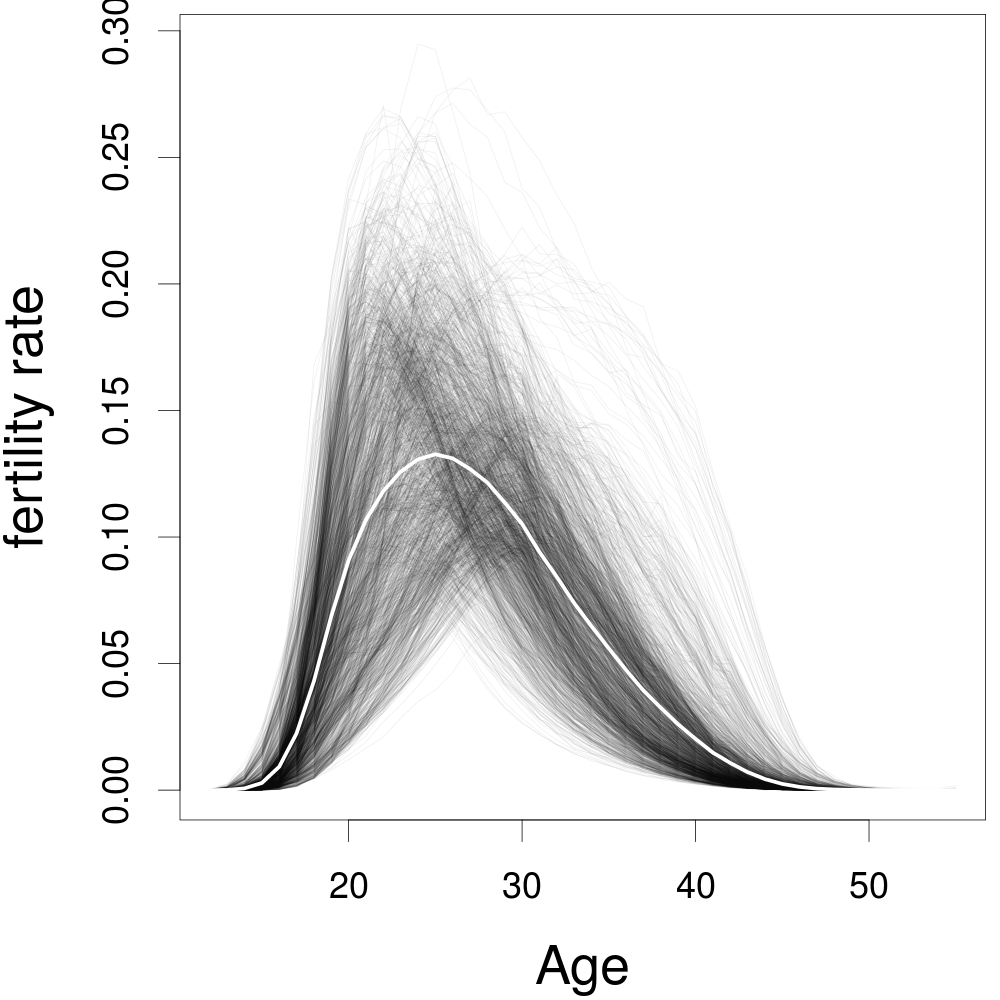
\includegraphics[height=6in]{Figures/Fertility2.png}
\end{center}
\end{frame}


\begin{frame}
\frametitle{laws for fertility}
\vspace{-1em}
\begin{center}
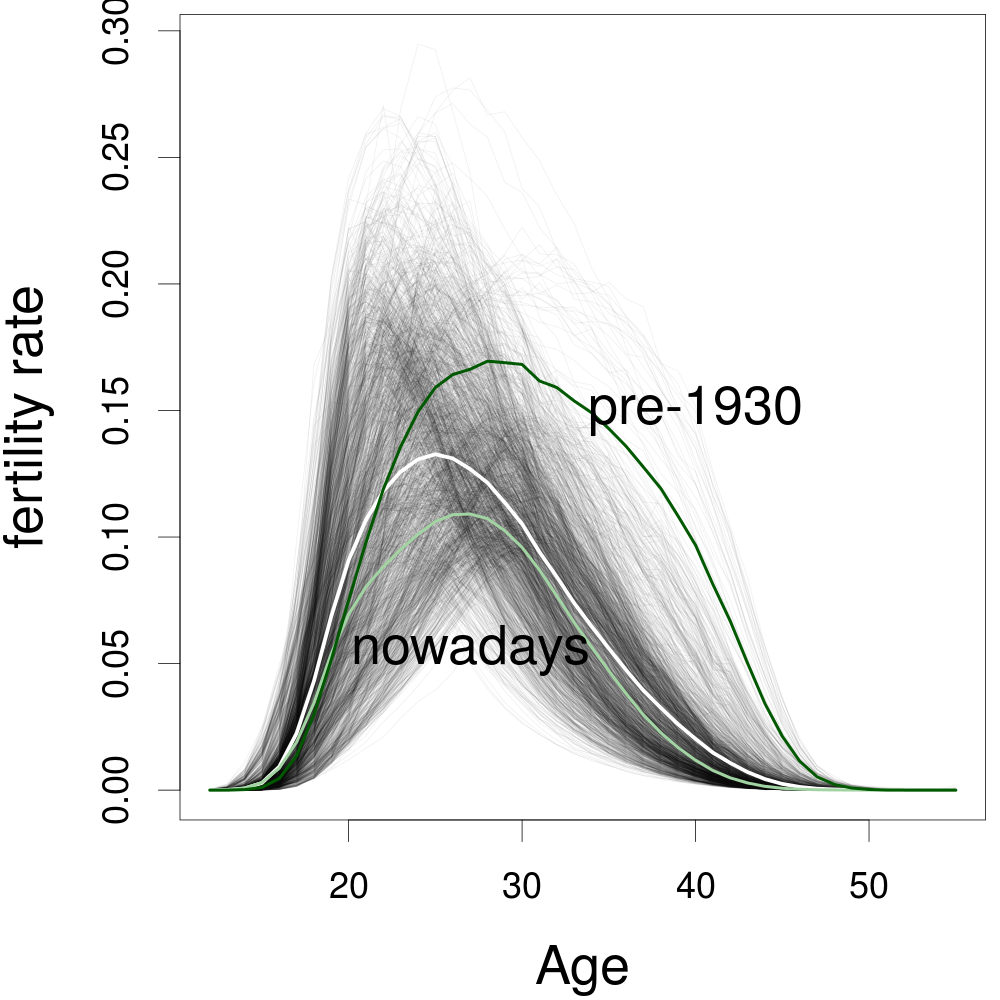
\includegraphics[height=6in]{Figures/Fertility3.png}
\end{center}
\end{frame}

\begin{frame}
\frametitle{laws for fertility: Sex ratio at birth}
\vspace{-2em}
\begin{center}
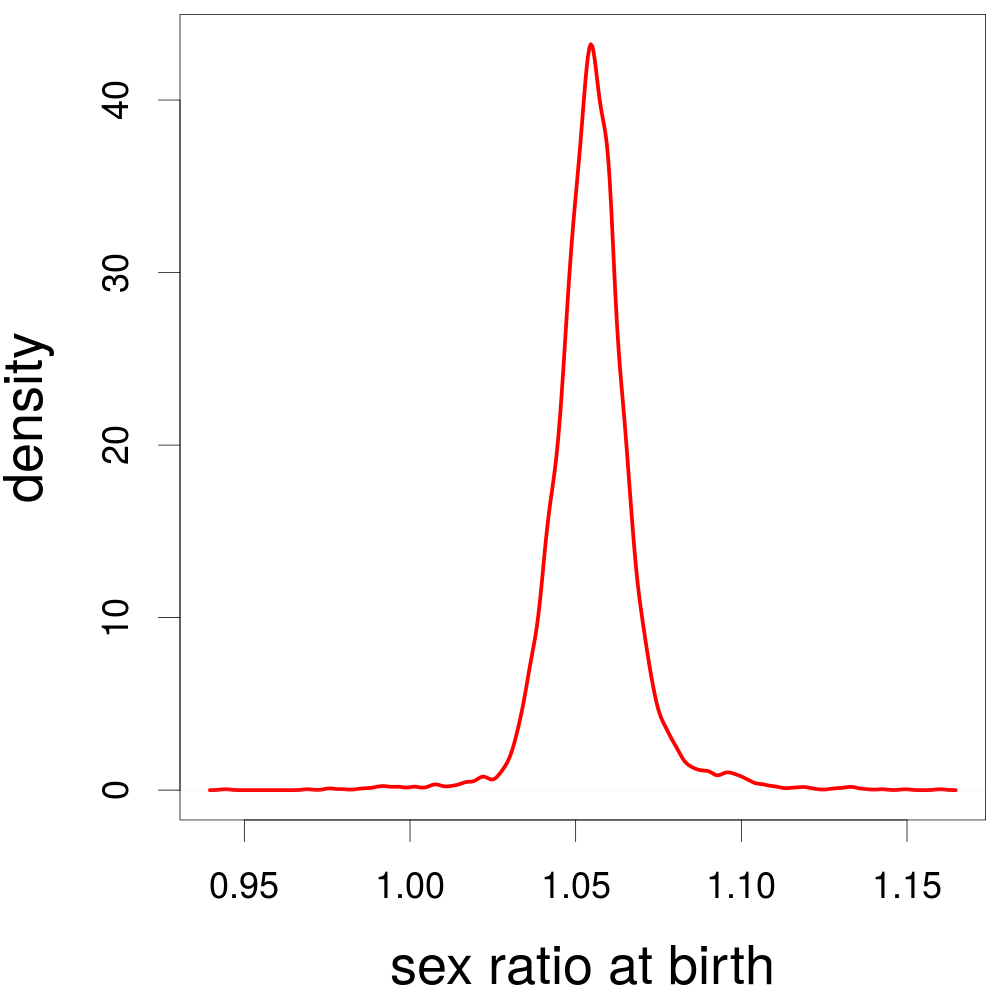
\includegraphics[height=6in]{Figures/SRB.png}
\end{center}
\end{frame}

\begin{frame}
\frametitle{continuous and discrete time}
\onslide<1>\begin{block}{On the one hand}
Populations are composed of a finite number of individuals. Events (birth,
death) are usually observed in discrete intervals. Problem for differentiable
equations for things?
\end{block}
\vspace{1em}
\onslide<2>\begin{block}{On the other hand}
We can think of underlying risk as a continuous and smooth function. And we can
think of population processes in the limit as continuous functions. Plus
continuous math is easier on the eyes.
\end{block}
\end{frame}

\begin{frame}
\frametitle{Models of understanding}
\vspace{-2em}
\begin{center}
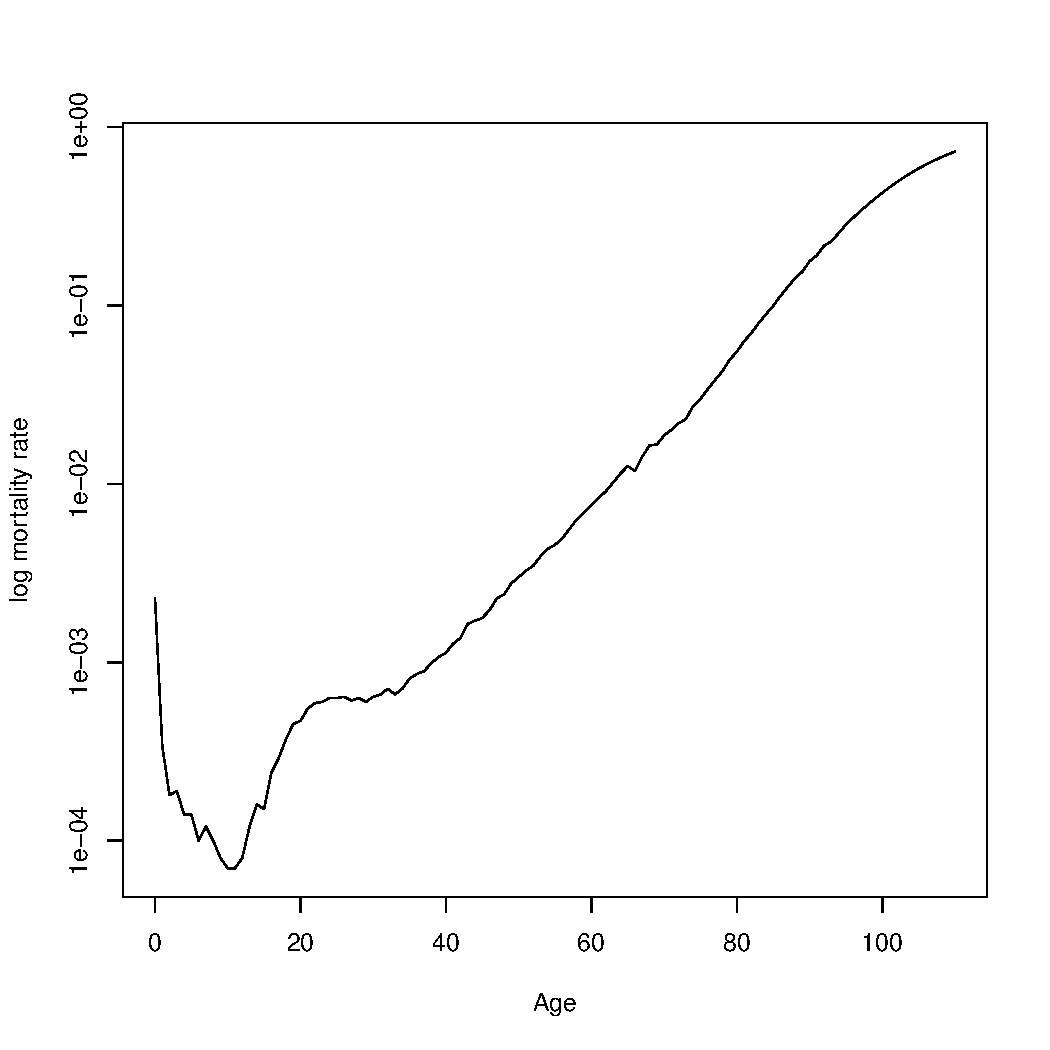
\includegraphics{Figures/MortalityGeneral1.pdf}
\end{center}
\end{frame}

\begin{frame}
\frametitle{Models of understanding}
\vspace{-2em}
\begin{center}
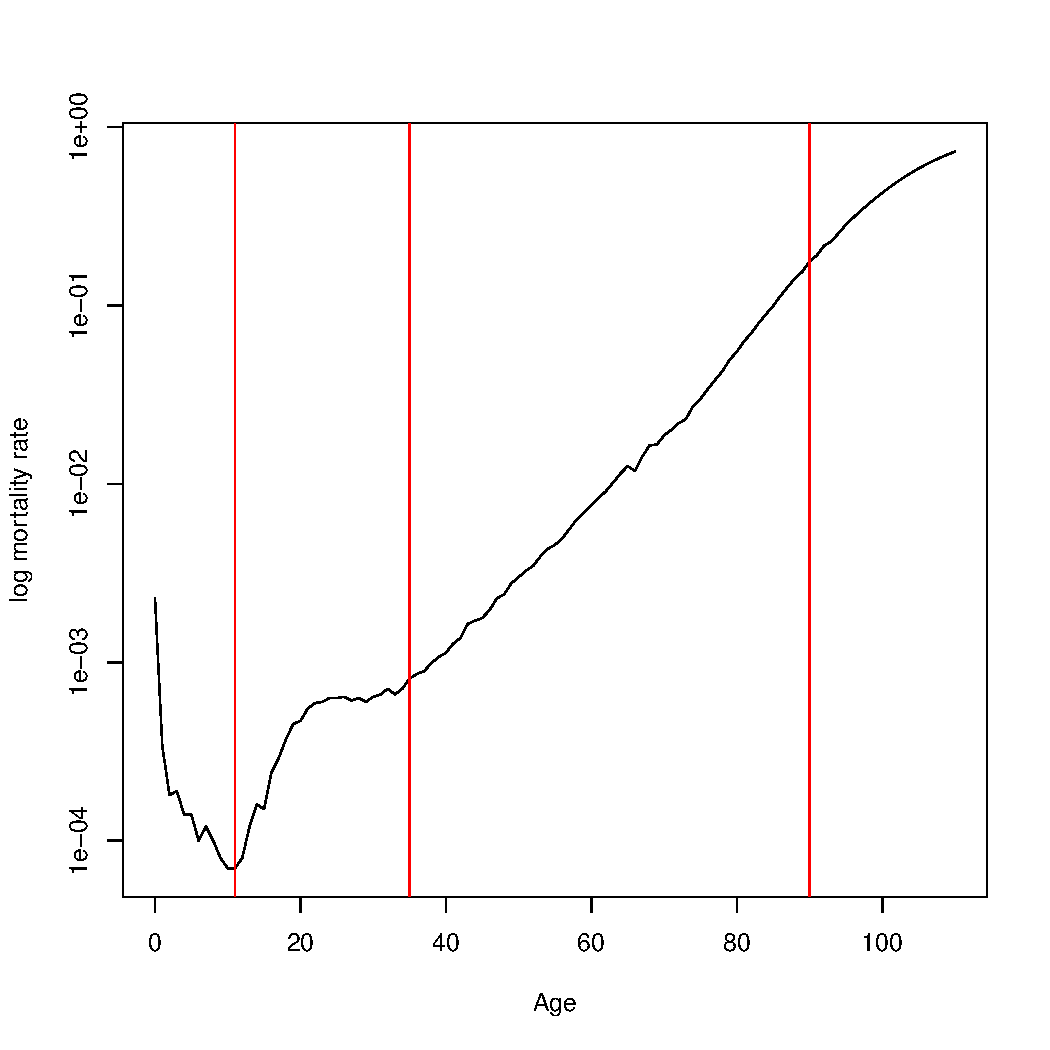
\includegraphics{Figures/MortalityGeneral2.pdf}
\end{center}
\end{frame}

\begin{frame}
\frametitle{Models of understanding: frailty}
\vspace{-2em}
\begin{center}
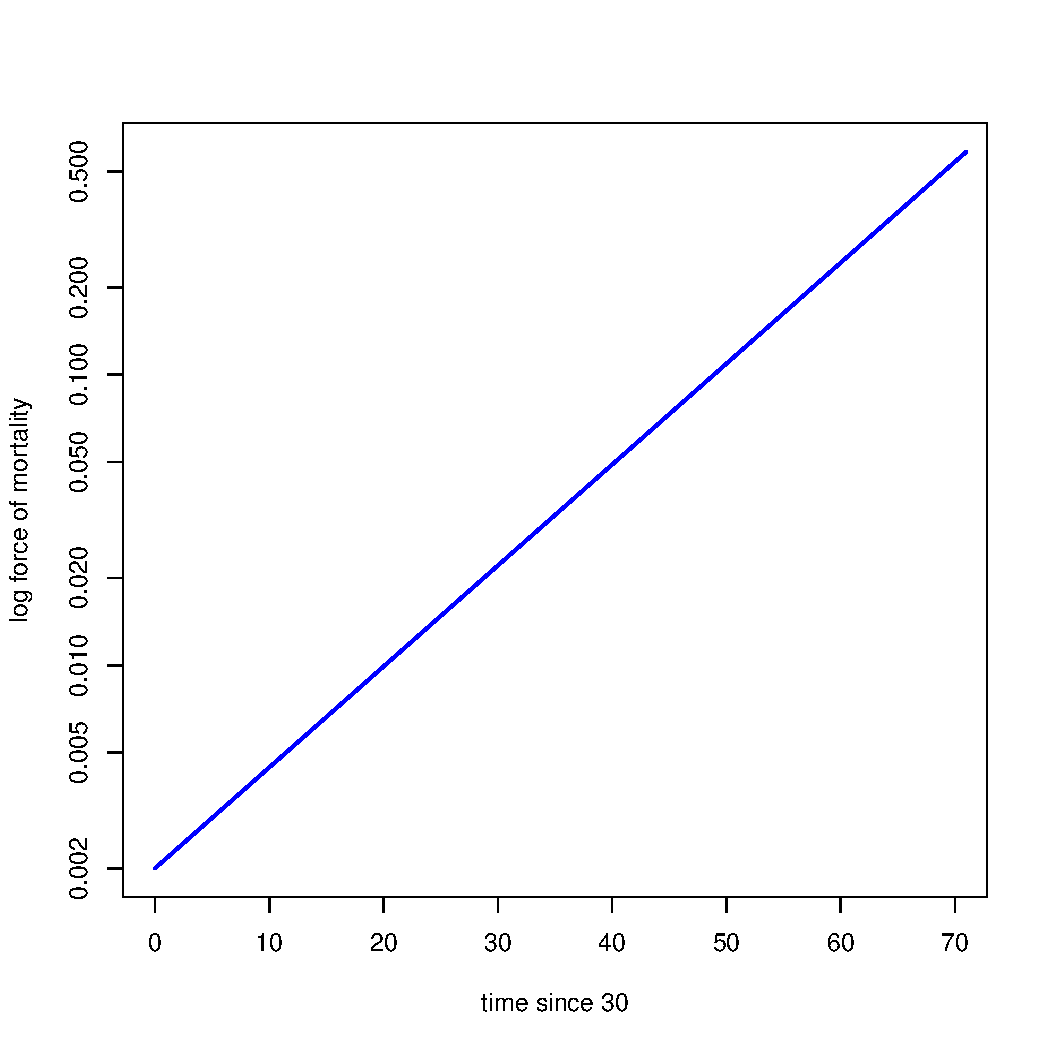
\includegraphics{Figures/Frailty1.pdf}
\end{center}
\end{frame}

\begin{frame}
\frametitle{Models of understanding: frailty}
\vspace{-2em}
\begin{center}
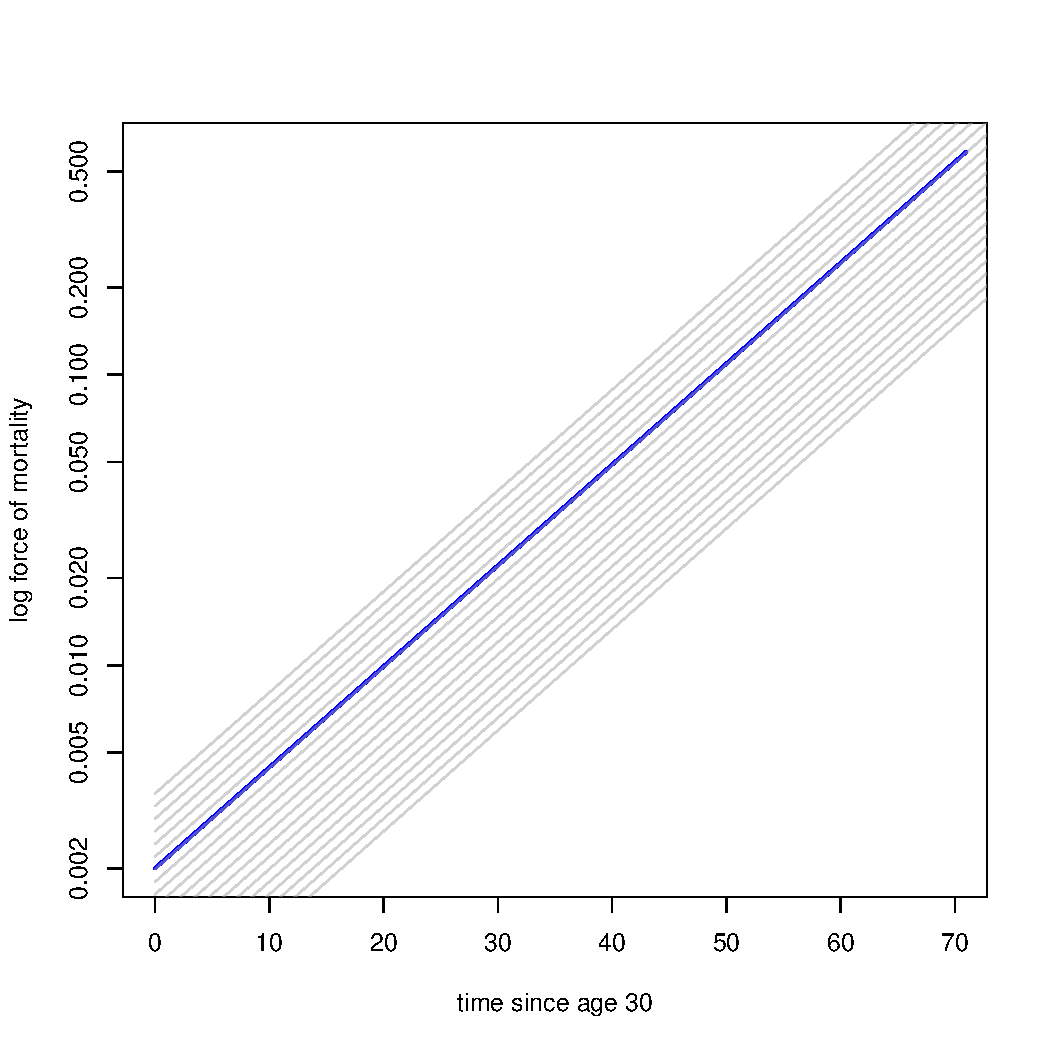
\includegraphics{Figures/Frailty2.pdf}
\end{center}
\end{frame}

\begin{frame}
\frametitle{Models of understanding: frailty}
\vspace{-2em}
\begin{center}
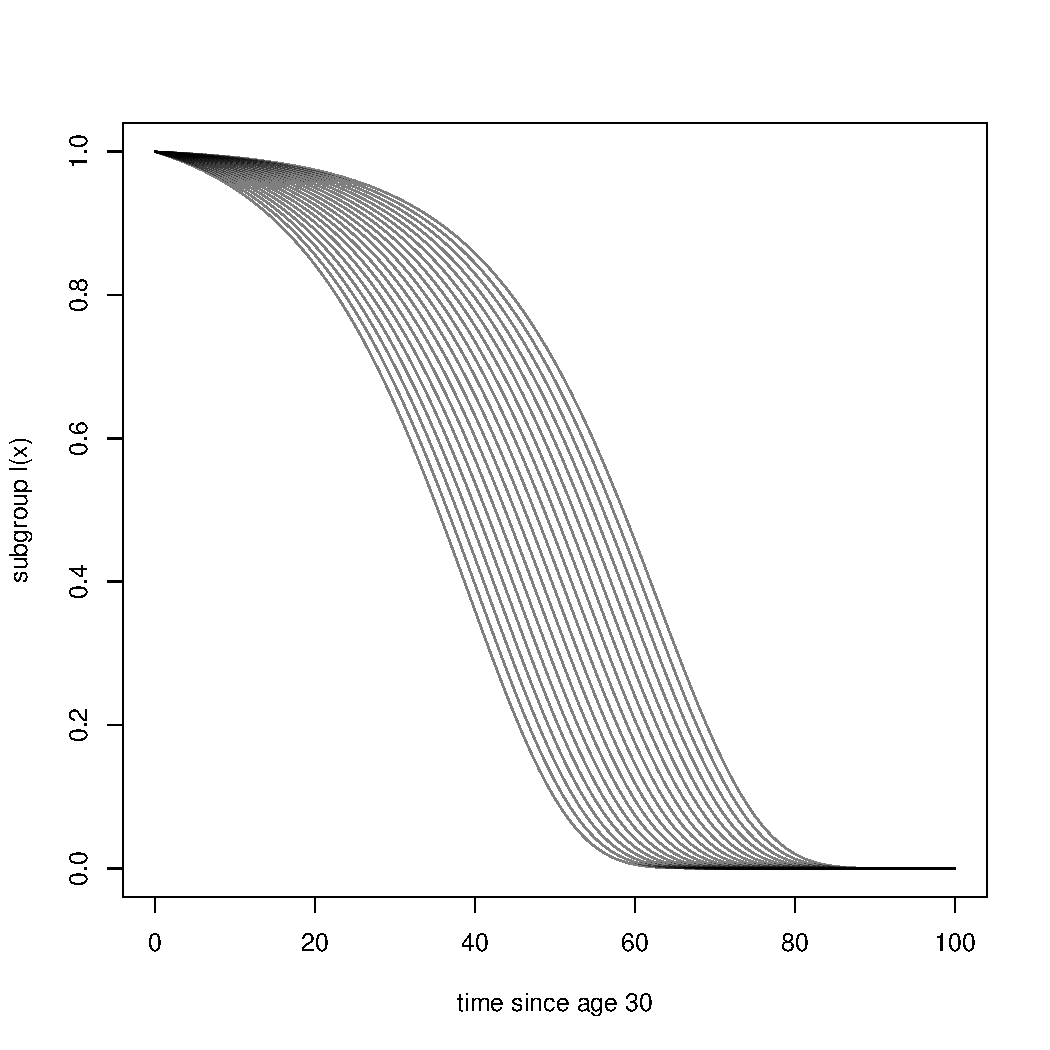
\includegraphics{Figures/Frailty3.pdf}
\end{center}
\end{frame}

\begin{frame}
\frametitle{Models of understanding: frailty}
\vspace{-2em}
\begin{center}
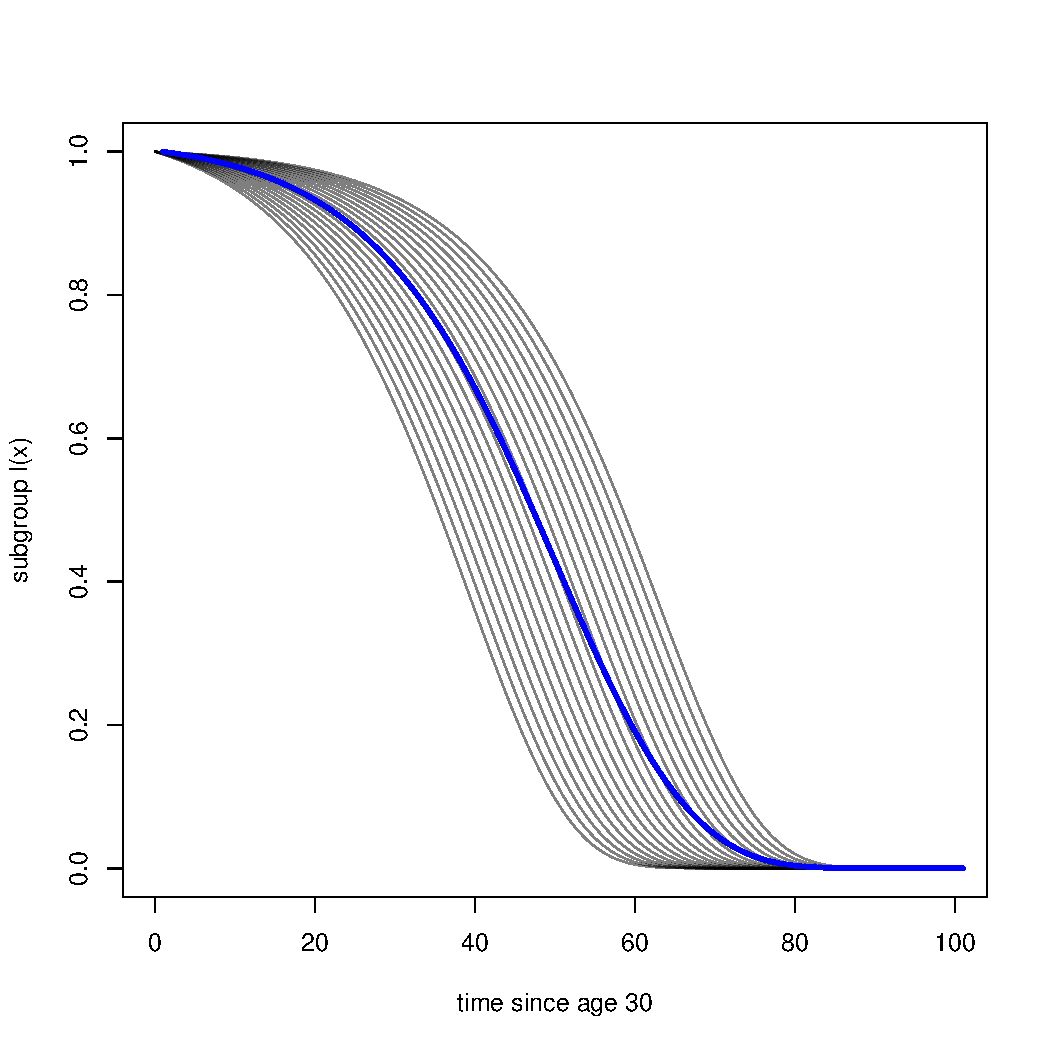
\includegraphics{Figures/Frailty4.pdf}
\end{center}
\end{frame}

\begin{frame}
\frametitle{Models of understanding: frailty}
\vspace{-2em}
\begin{center}
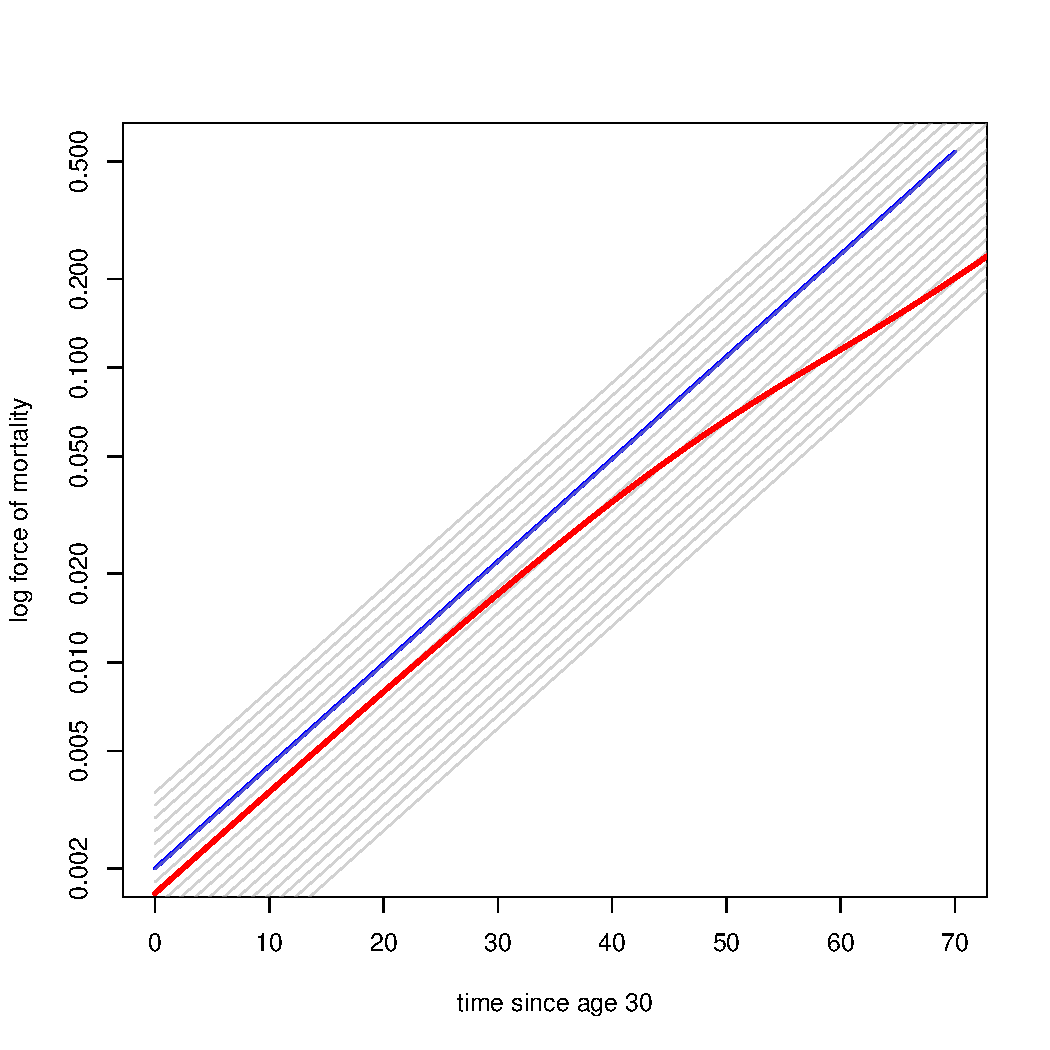
\includegraphics{Figures/Frailty5.pdf}
\end{center}
\end{frame}

\begin{frame}
\frametitle{Models of understanding: and yes, there's math}
\vspace{-2em}
\begin{center}
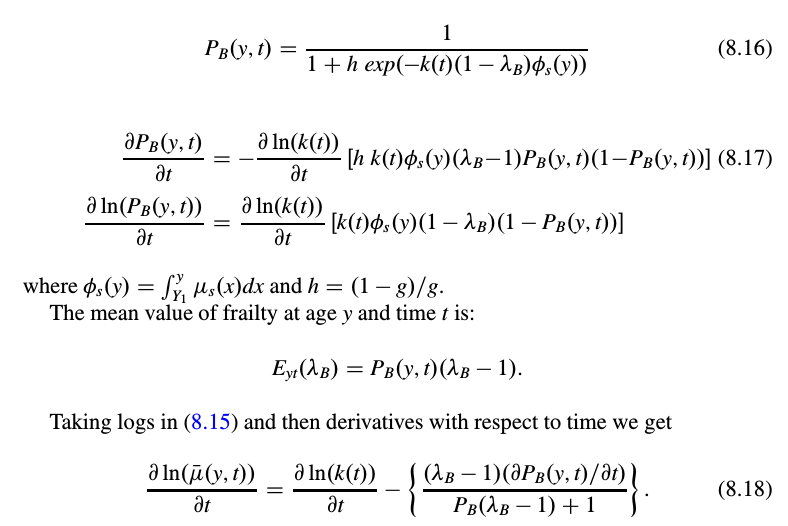
\includegraphics[height=5in]{Figures/PalloniShot.png}
\end{center}
\color{mygray}{screenshot from Palloni \& Beltran-Sanchez (2016)}
\end{frame}

\begin{frame}
\frametitle{Population renewal}
\vspace{-2em}
\begin{center}
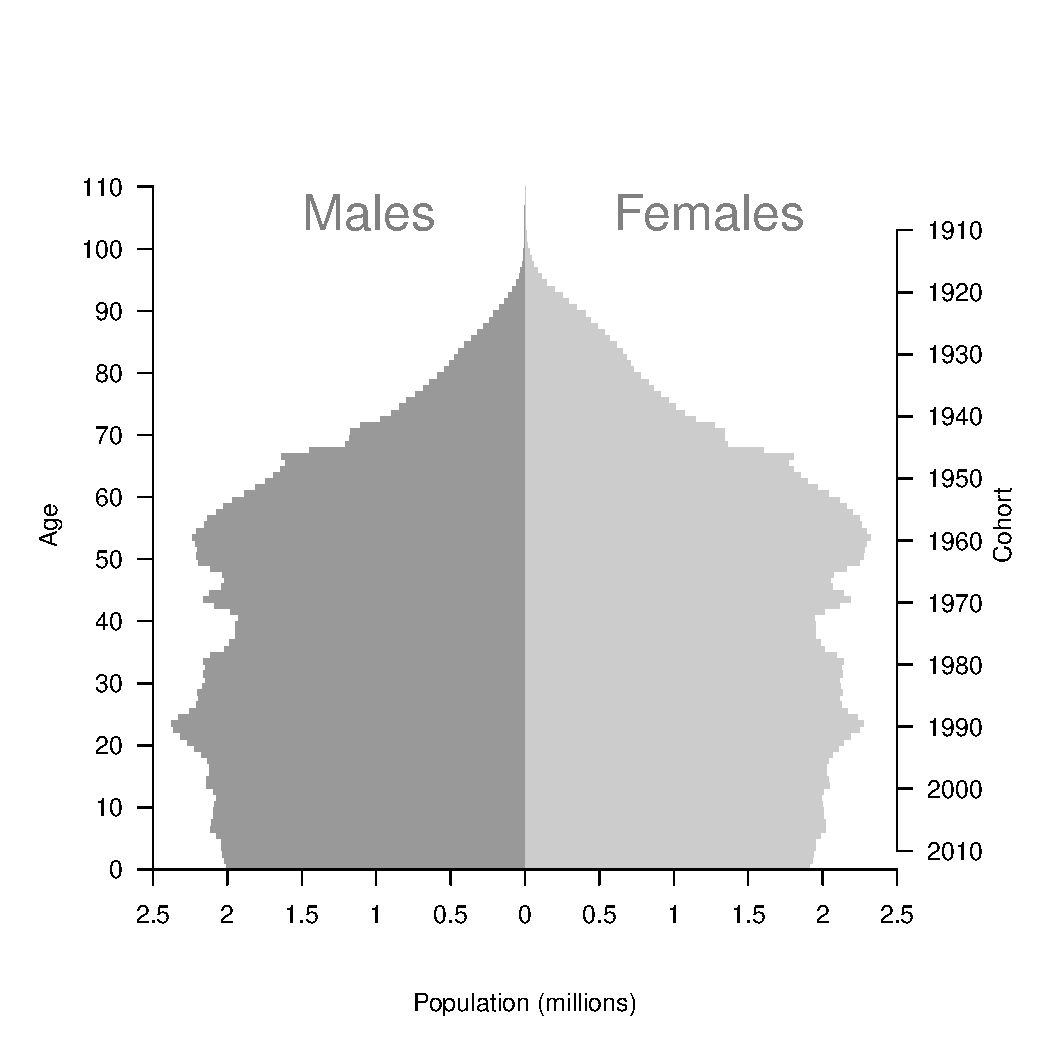
\includegraphics[height=7in,trim=20 20 20 20]{Figures/PopUSA2014.pdf}
\end{center}
\end{frame}

\begin{frame}
\frametitle{Population renewal}
\vspace{-2em}
\begin{center}
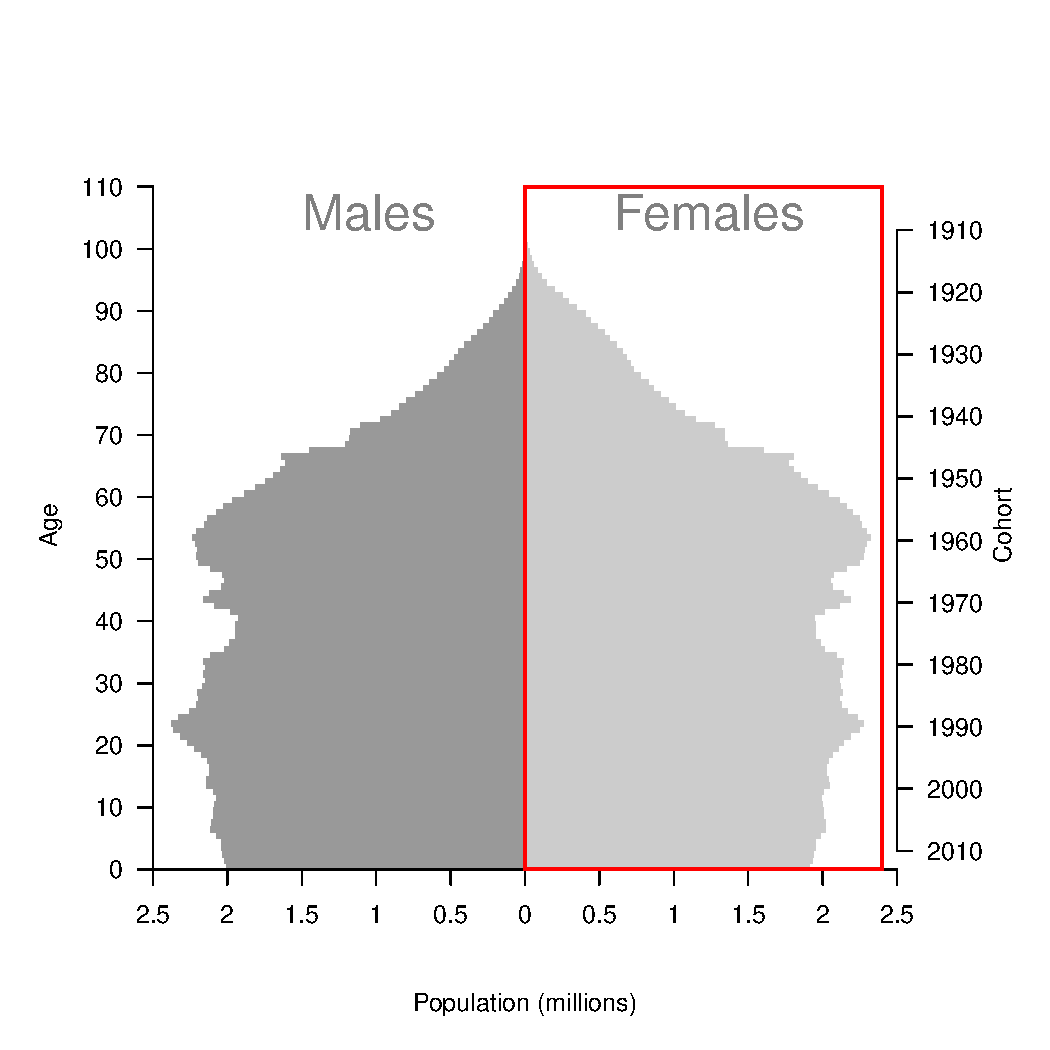
\includegraphics[height=7in,trim=20 20 20 20]{Figures/PopUSA20142.pdf}
\end{center}
\color{mygray}{This is where I explain renewal by waving my hands around. Ask
for equations if that helps!}
\end{frame}

\begin{frame}
\frametitle{Population renewal}
\vspace{-2em}
\begin{center}
\animategraphics{15}{Figures/Animation/P}{1}{187}
%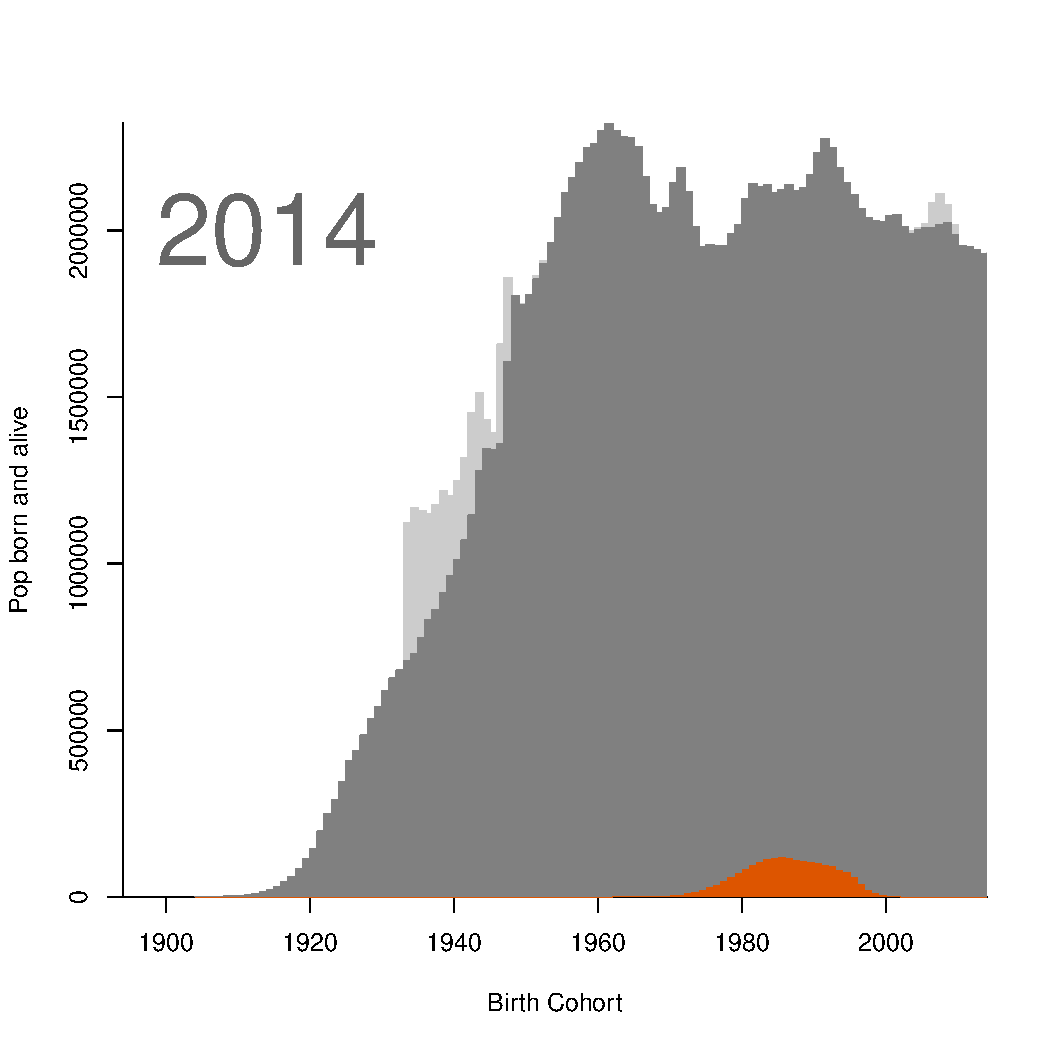
\includegraphics{Figures/Animation/P1.pdf}
\end{center}
\end{frame}

\begin{frame}
\frametitle{more math in demography}
\begin{itemize}[<+->]
  \item indirect methods of estimation: requires models
  \item data quality control: requires models
  \item models of interactions, contagion, mixing: populations are heterogeneous
  \item models of health and disease transitions
  \item parametric models of mortality and fertility
  \item Math is at the core of demography
\end{itemize}
\end{frame}

\begin{frame}
\frametitle{where can you get paid to do this stuff?}
\begin{itemize}[<+->]
  \item the Census Bureau, CDC, NIH, State govs
  \item academia: Berkeley, Princeton, Penn, IHME
  \item private and international research: Rand corp, World Bank, UN
  \item insurance companies (major crossover with actuarial science)
\end{itemize}
\color{mygray}{feel free to inquire about coming to Rostock, Germany to geek out
in mathematical demography}
\end{frame}
\end{document}
